  \section{Marco Teórico}

    Realizar análisis de señales en dominio de la frecuencia, posee la ventaja de poder 
    brindar mas información a diferencia de hacerlo bajo el dominio del tiempo. 
    Por ejemplo, se puede visualizar una onda senoidal en el tiempo ,entregada 
    por un generador de funciones, con un osciloscopio y notar una distorsión muy leve 
    en sus picos, casi imperceptible, lo cual, si dicha señal se la analizara bajo el 
    dominio de la frecuencia, quedaría en evidencia clara que la misma no es una señal 
    senoidal pura sino que posee armónicos debido al modo que utilizan los generadores 
    de funciones para crear dicha señal.
    
    La desventaja de analizar señales en el 
    dominio de la frecuencia es que no se puede obtener información de la fase relativa de 
    la señal bajo análisis, solo es posible obtener la amplitud de las componentes
    espectrales. La otra desventaja a destacar es que, resulta difícil realizar análisis de 
    transitorios rápidos, estos mismos son mas cómodos de analizar en el dominio del tiempo.
    
    Para el presente trabajo practico se realizará los ensayos con un osciloscopio digital 
    el cual posee un modulo matemático (\textbf{Math menu}) que cuenta con la transformada 
    rápida de Fourier (FFT). 

    \subsubsection{Analizador de Fourier }
    
    El analizador de fourier, posee un conjunto de filtros donde cada uno de los 
    mismos se encuentran ligeramente desfasados entre si y repartidos de manera 
    uniforme sobre el margen de frecuencia que se desea analizar, tal como se observa
    en la Figura~\ref{fig:EsqInicialFourier}. El conjunto de filtros puede formar 
    parte de un sistema mas complejo, donde sus salidas pueden ser multiplexadas 
    y mostradas en conjunto con un amplificador vertical en una pantalla y a su ves, 
    el multiplexor con un contador, aparte de seleccionar el conjunto de filtros, 
    generar una señal de rampa escalera para posteriormente pasar por un 
    amplificador horizontal y realizar un barrio de eje horizontal de la pantalla 
    para poder visualizar el espectro en frecuencia de una señal. En la 
    Figura~\ref{fig:EsqAnalizadorDeFourierBasico}, se muestra un diagrama en bloques 
    simplificado de un analizador de fourier el cual, su principal 
    ventaja es que, el análisis se hace practicamente en forma simultánea en todo 
    el espectro. Pero dichos instrumentos poseen como desventaja una excesiva 
    complejidad del sistema y a su vez poseen baja resolución con un \textit{spam} 
    (margen de frecuencia de trabajo) fijo.
    \begin{figure}[H]
        \centering
        \begin{subfigure}[H]{0.48\textwidth}
          \frame{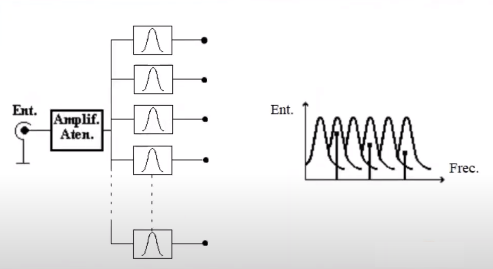
\includegraphics[width=\textwidth]{Imagenes/MarcoTeorico/EsqInicialAnalizDeFourier.png}}
          \caption{Conjunto de Filtros.}
          \label{fig:EsqInicialFourier}
        \end{subfigure}
        \hfill 
        \begin{subfigure}[H]{0.45\textwidth}
          \frame{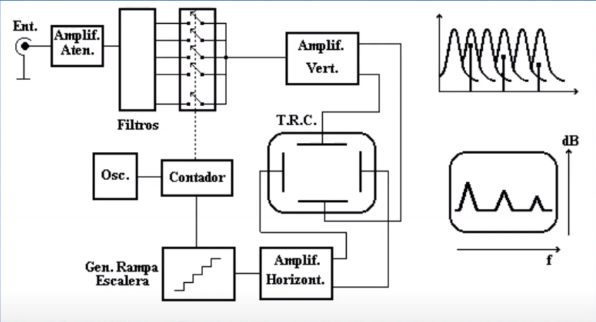
\includegraphics[width=\textwidth]{Imagenes/MarcoTeorico/EsqDeAnalizadorDeFourierBasico.png}}
          \caption{Esq. en bloques simplificador.}
          \label{fig:EsqAnalizadorDeFourierBasico}
        \end{subfigure}
        \caption{Analizar de fourier básico.}
        \label{fig:AnalizadorDeFourier}
      \end{figure}
           
    \subsubsection{Módulo matemático en Osciloscopios Digitales}

    Con la llegada de los osciloscopios digitales con módulo matemático, estos mismos 
    fueron reemplazando los analizadores de fourier convencionales.
    Dicho módulo posee un algoritmo de transformada rápida de fourier (FFT), donde 
    a partir de las muestras tomadas en el dominio del tiempo de una señal de entrada,
    se realiza la conversion de la señal con la FFT al dominio de la frecuencia.
    El esquema en bloques simplificado se puede observar en la Figura~\ref{fig:MathModuleEnOscil}.
        \begin{figure}[H]
            \centering
            \frame{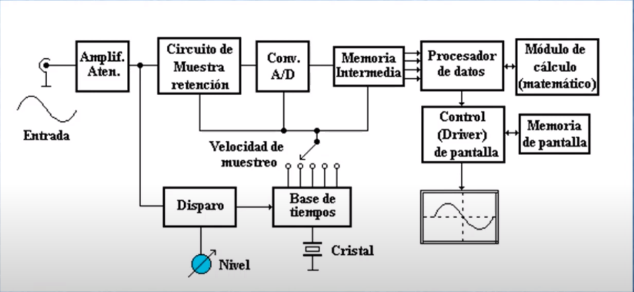
\includegraphics[width=\textwidth]{Imagenes/MarcoTeorico/MathModuleEnOscilDigital.png}}
            \caption{Módulo matemático en Osciloscopio Digital.}
            \label{fig:MathModuleEnOscil}
        \end{figure}
    
    En el modelo de Osciloscopio utilizado en el presente trabajo práctico (TP) 
    (\textit{Tektronix TDS 1001}), cuya presentación de pantalla se observa en la 
    Figura~\ref{fig:MathModoEnTek}.   
        \begin{figure}[H]
            \centering
            \frame{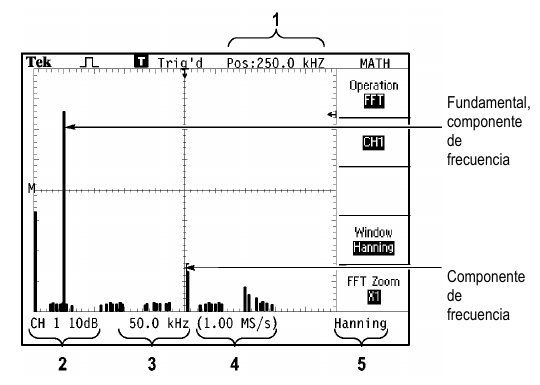
\includegraphics[width=\textwidth]{Imagenes/MarcoTeorico/PresentacionDePantallaFFT.png}}
            \caption{Modo Matemático en Osciloscopio,}
            \label{fig:MathModoEnTek}
        \end{figure}
    Donde se destaca los siguientes puntos 
    \begin{enumerate}
        \item Frecuencia de la linea central de la pantalla.
        \item Escala Vertical en dB/div donde (0 dB = 1 \(V_{RMS}\)).
        \item Escala horizontal en Frec/div.
        \item Velocidad de muestreo. 
        \item Tipo de ventana FFT. 
    \end{enumerate}    

     A continuación, se hace incapie en los tipos de ventanas que se utilizaran en el 
     presente TP como se observa en la Figura~\ref{fig:VentanasTipos} indicando sus 
     ventajas y desventajas.
        \begin{figure}[H]
            \centering
            \begin{subfigure}[H]{0.45\textwidth}
            \frame{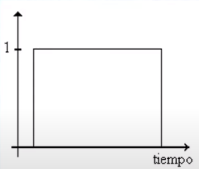
\includegraphics[width=\textwidth]{Imagenes/MarcoTeorico/VentanaRectangular.png}}
            \caption{Ventana Rectangular.}
            \label{fig:VentanaRec}
            \end{subfigure}
            \hfill 
            \begin{subfigure}[H]{0.45\textwidth}
            \frame{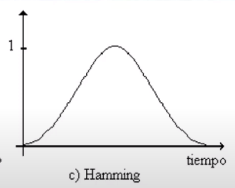
\includegraphics[width=\textwidth]{Imagenes/MarcoTeorico/VentanaHamming.png}} 
            \caption{Ventana Hamming.}
            \label{fig:VentanaHamming}
            \end{subfigure}
            \hfill 
            \begin{subfigure}[H]{0.45\textwidth}
            \frame{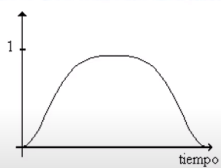
\includegraphics[width=\textwidth]{Imagenes/MarcoTeorico/VentanaFlattop.png}}
            \caption{Ventana flattop.}
            \label{fig:VentanaFlattop}
            \end{subfigure}

            \caption{Tipos de Ventan para FFT.}
            \label{fig:VentanasTipos}
        \end{figure}
    
    La \textbf{ventana rectangular}, Figura~\ref{fig:VentanaRec} posee como principal ventaja que son
    de gran utilidad para medir señales que poseen transitorios rápidos.
    como la ventana rectangular es una ventana de apertura y cierre abrupto, esto puede generar
    la aparición a flancos abruptos que no existen realmente en la señal, causando errores 
    en la lectura de la misma.
    
    La \textbf{ventana Hamming}, Figura~\ref{fig:VentanaHamming} se las concidera como una ventana de 
    apertura y cierre suave a diferencia de la rectangular. Esto permite eliminar el problema
    de los flancos abruptos facilitando las mediciones de amplitudes de las componentes 
    espectrales de una señal, pero como desventaja poseen poca exactitud para realizar 
    mediciones de frecuencias.
    
    Por último la \textbf{ventana flattop}, Figura~\ref{fig:VentanaFlattop} es una solución de compromiso
    entre las dos ventanas previamente mencionadas. 

    \subsubsection*{Uso de Cursores}
        
        Cabe destacar, que también se para realizar las mediciones en los diferentes ensayos
        se utiliza los \textbf{cursores} propios del osciloscopio. Con ellos se puede 
        realizar mediciones en amplitud (dB) o frecuencia tal como se observa en la
        Figura~\ref{fig:CursorTipos}.  
            \begin{figure}[H]
                \centering
                \begin{subfigure}[H]{0.45\textwidth}
                \frame{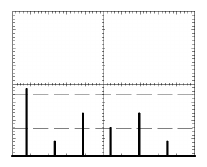
\includegraphics[width=\textwidth]{Imagenes/MarcoTeorico/CursoresEnMagnitud.png}}
                \caption{Cursores en Magnitud.}
                \label{fig:CursorMag}
                \end{subfigure}
                \hfill 
                \begin{subfigure}[H]{0.45\textwidth}
                \frame{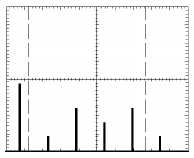
\includegraphics[width=\textwidth]{Imagenes/MarcoTeorico/CursoresEnFrecuencia.png}}
                \caption{Cursores en Frecuencia.}
                \label{fig:CursorFrec}
                \end{subfigure}
                \caption{Tipos de cursores del Osciloscopio Digital.}
                \label{fig:CursorTipos}
            \end{figure}

        Se debe tener presente que cuandos e realiza mediciones en magnitud en frecuencia con 
        el osciloscopio, dicha magnitud dada en decibleles esta referenciada a valor de RMS
        y no de amplitud pico de la señal.
                
    

    








